\documentclass{estilo}
\usepackage[spanish]{babel}
\usepackage{graphicx}
\usepackage{float}
\usepackage{amsmath}        % para los vectores columnas
\usepackage{amsfonts}       % para las negrita de pizarra
\usepackage{amssymb}        % para simbolos matematicos
\usepackage{amsmath}        % para los vectores columnas
\usepackage{hyperref}       % para utilizar referencias
\usepackage{multirow}       % para las tablas
\usepackage{dsfont}
\usepackage{listings}
\usepackage{xcolor}
\usepackage{hyperref}

\usepackage{tocloft}

\definecolor{codegreen}{rgb}{0,0.6,0}
\definecolor{codegray}{rgb}{0.5,0.5,0.5}
\definecolor{codepurple}{rgb}{0.58,0,0.82}
\definecolor{backcolour}{rgb}{0.95,0.95,0.92}
\lstdefinestyle{mystyle}{
    backgroundcolor=\color{backcolour},   
    commentstyle=\color{codegreen},
    keywordstyle=\color{magenta},
    numberstyle=\tiny\color{codegray},
    stringstyle=\color{codepurple},
    basicstyle=\ttfamily\footnotesize,
    breakatwhitespace=false,         
    breaklines=true,                 
    captionpos=b,                    
    keepspaces=true,                 
    numbers=left,                    
    numbersep=5pt,                  
    showspaces=false,                
    showstringspaces=false,
    showtabs=false,                  
    tabsize=2
}
\lstset{style=mystyle}

\usepackage{enumitem,multicol,setspace}
\newcounter{subenum}[enumi] % para las multicolumnas
\renewcommand{\thesubenum}{\arabic{subenum}}
\usepackage[nomessages]{fp}
\FPeval\thecolwidth{round(1/4:4)}% Specify number of columns -> column width
\newcommand{\newitem}[1]{%
  \refstepcounter{subenum}%
  \parbox{\dimexpr\thecolwidth\linewidth-.5\columnsep}{%
    \makebox[\labelwidth][r]{(\thesubenum)\hspace*{\labelsep}}%
    #1}\hfill%
}

\usepackage{scalerel,stackengine} % para el sombrero
\stackMath
\newcommand\rhat[1]{%
\savestack{\tmpbox}{\stretchto{%
  \scaleto{%
    \scalerel*[\widthof{\ensuremath{#1}}]{\kern-.6pt\bigwedge\kern-.6pt}%
    {\rule[-\textheight/2]{1ex}{\textheight}}%WIDTH-LIMITED BIG WEDGE
  }{\textheight}% 
}{0.5ex}}%
\stackon[1pt]{#1}{\tmpbox}%
}
\parskip 1ex

\usepackage{mathtools}      % floor y ceil
\DeclarePairedDelimiter\ceil{\lceil}{\rceil}
\DeclarePairedDelimiter\floor{\lfloor}{\rfloor} 

\usepackage[style=authoryear-comp]{biblatex}


\begin{document}

\maketitle

\newpage

\tableofcontents

\newpage

\section{Introducción}

En el presente informe, se tiene como objetivo llevar a cabo un análisis del diseño 
implementado para abordar la problemática planteada por Scaloni, que consiste en la 
optimización máxima del tiempo total empleado en la realización de un análisis exhaustivo 
de sus rivales. A lo largo de este, se expondrán los criterios empleados y se proporcionará 
su justificación.


\subsection{Información de la problemática}

El enunciado propuesto, nos da la siguiente información:

\begin{itemize}

    \item Cada compilado lo debe analizar Scaloni y alguno de sus ayudantes.

    \item El análisis del rival $i$ le toma $s_i$ tiempo a Scaloni y luego $a_i$ tiempo al ayudante.
    
    \item Al momento en que Scaloni haya terminado de analizar el $i$ ésimo compilado, comenzará
    inmediatamente algún ayudante a analizarlo, para no desperdiciar ningún segundo.

    \item Scaloni cuenta con $n$ ayudantes, siendo $n$ la cantidad de rivales a analizar. Además, cada
    ayudante puede ver los compilados completamente en paralelo a Scaloni y a los respectivos ayudantes.

    \item Sólo un ayudante verá el compilado, dado que no aporta mayor ganancia que dos ayudantes lo vean.

\end{itemize}

/section{Análisis de la complejidad del problema}

El problema planteado por Scaloni se enmarca como un caso específico del problema del 
Hitting-Set, cuya definición formal se presenta de la siguiente manera: dado un 
conjunto $A$ compuesto por $n$ elementos y $m$ subconjuntos $B_{1}, B_{2}, \dots, B_{m}$ 
pertenecientes a $A$ ($B_{i}\subseteq A \forall i \in \mathbb{N}_{m}$), se busca encontrar un conjunto $C \subseteq A$ tal que para cada 
subconjunto $C$, donde $C \subseteq A / \forall j \in \mathbb{N}_{m},  C \cap B_{j}\neq \emptyset$. 

Además de su formulación básica, el problema del Hitting-Set también presenta una versión
de decisión: dada la colección de un conjunto $A$ con $n$ elementos y $m$ subconjuntos
 $B_{1}, B_{2}, \dots, B_{m}$ de $A$ ($B_{i}\subseteq A$ para cada $i$), junto con un 
 parámetro numérico $k$, se plantea el interrogante sobre la existencia de un conjunto 
 $C \subseteq A$ que cumpla con dos condiciones fundamentales:
 \item En primer lugar, que la cardinalidad de $C$ sea menor o igual a $k$ ($\left| C \right|\leq k$) 
 \item En segundo lugar, que para cada subconjunto $B_{j}$, la intersección entre $C$ y $B_{j}$ no sea 
 vacía ($C \cap B_{j} \neq \emptyset$) para todo $j$ perteneciente al conjunto de 
 números naturales hasta $m$.

El problema del Hitting-Set se sitúa en la clase de complejidad NP debido a su capacidad 
de verificación en tiempo polinomial, lo que implica una verificación eficiente de su 
solución propuesta. La verificación de la solución se reduce a confirmar dos condiciones 
fundamentales: Primero, se debe comprobar que la cardinalidad del conjunto propuesto $C$ 
es menor o igual a $k$, donde $k$ es un parámetro dado. Segundo, es necesario 
verificar que para cada conjunto $B_{j}$ dentro de una colección de subconjuntos 
$B_{1}, B_{2}, \dots, B_{m}$, $C$ contenga al menos un elemento de $B_{j}$.

Para realizar esta verificación, se llevan a cabo dos operaciones clave que definen la 
complejidad del proceso. La primera operación, relacionada con la verificación de la 
cardinalidad de $C$ ($\left| C \right|\leq k$), tiene una complejidad constante $O(1)$, 
ya que implica simplemente obtener el número de elementos en $C$ y verificar que $#C \leq k$.

La segunda operación, que implica verificar la inclusión de al menos un elemento de $C$ 
en cada conjunto $B_{j}$, presenta una complejidad de $O(n \times m)$. Esto se debe a 
que para cada conjunto $B_{j}$ ($j$ perteneciente al conjunto de números naturales hasta 
$m$) (operación $O(m)$), se debe recorrer, en el peor de los casos, todo el conjunto $C$ 
($O(n)$) para verificar la pertenencia de al menos un elemento de este en $B_{j}$ 
(operación con complejidad $O(1)$ si tanto $B_{j}$ como $C$ se implementan como un conjunto 'set').

La clasificación del problema del Hitting-Set como NP-Completo se establece mediante la demostración
de su reducibilidad polinómica a partir de otros problemas ya catalogados como NP-Completo. 

En nuestro análisis, nos hemos propuesto abordar esta demostración de dos maneras distintas, 
empleando estrategias de reducción que ilustran la naturaleza NP-Completa del Hitting-Set Problem:

\item Reducción de Vertex Cover a Dominating-Set Problem -> Reducción de Dominating-Set Problem a Hitting-Set Problem.
\item Reducción de Set Cover a Hitting-Set Problem.


/subsection{Reducción Vertex Cover a Dominating-Set Problem}
La reducción $\text{Vertex-Cover} \leq _{p} \text{Dominating-Set}$ consta en lo siguiente:
Dado del grafo $G$ con $n$ vértices y $m$ aristas del problema Vertex Cover, para cada par de 
vértices adyacentes $v-w$, se agregan ambos al grafo $G'$ (del problema Dominating Set) junto a 
su arista y se agrega un tercer vértice auxiliar $vw$, adyacente a los otros dos. $A$ será el 
conjunto de vértices auxiliares. Luego, del conjunto $V'$ de $k$ vértices solución de 
Dominating Set, se debe agregar a $V$ (solución de Vertex Cover) todos los vértices de $V'$ que 
no estén en el conjunto de auxiliares y, para cada vértice en $V' \cap A$ se agrega a $V$ 
cualquiera de sus adyacentes. La primera parte de la reducción es $O(m)$ y la segunda es 
$O(k),k \leq n$, por lo que la complejidad total es $O(m+k)$, que es polinomial.

\[\text{Vertex-Cover} \leq _{p} \text{Dominating-Set}\]

% Gráficos ej de reducción

Finalmente:

\[
    \begin{array}{c}
        \begin{split}
            \text{Vertex-Cover}  & \leq _{p} \text{Dominating-Set} \\
            \text{Dominating-Set}  & \leq _{p} \text{Hitting-Set} \\
        \end{split}
        \quad \overset{ \text{por transitividad} }{ \implies  } \quad
        \text{Vertex-Cover}  \leq _{p} \text{Hitting-Set} \\ \\
        \implies \text{Hitting-Set} \in \text{NP-Completo}    
    \end{array}
\]



Es importante destacar que tanto Dominating-Set Problem como Set Cover han sido previamente establecidos
como problemas pertenecientes a la clase NP-Completo, hecho que fue demostrado en clases anteriores.



La estrategia de reducción polinómica propuesta tiene como objetivo evidenciar la equivalencia en 
términos de complejidad entre estos problemas conocidos y el Hitting-Set Problem, consolidando así 
la pertenencia de este último en la categoría de problemas NP-Completo.






Recordemos el problema de Dominating Set: Dado un grafo $G$, se busca un conjunto de vértices $C$
tal que, para todo vértice $v \in G$, este esté contenido en $C$ o existe al menos un vértice en $C$ adyacente de $v$.

La reducción $\text{Dominating-Set} \leq_{p} \text{Hitting-Set}$ consta en lo siguiente:
Dado un grafo $G$ de $n$ vértices del problema Dominating Set, Para cada vértice $v_{i}$, se construye un grupo $B_{i}$ con el mismo y todos sus vértices adyacentes. Entonces, el grupo resultado del Hitting Set con los subconjuntos $B_{1},B_{2},\dots,B_{m}$ será también el grupo resultado del Dominating Set. \textit{Nota: Para cada $k$-clique dentro del grafo habrá hasta $k$ sets iguales.} La complejidad de esta reducción depende de la implementación del grafo: Si los vértices desconocen a sus adyacentes, es $O(n^{2})$ porque para cada vértice $v_{i}$ se debe recorrer todos los vértices de $G$ para verificar si son adyacentes a $v_{i}$; en cambio, si los vértices tiene referencia a sus adyacentes, la complejidad es $O(n\times o)$, siendo $o$ el promedio del grado entre vértices, que puede variar entre $0$ y $m$. En ambos casos, se trata de una complejidad polinomial.

\[\text{Dominating-Set}  \leq _{p} \text{Hitting-Set}\]

% Gráficos ej de reducción

La reducción $\text{Vertex-Cover} \leq _{p} \text{Dominating-Set}$ consta en lo siguiente:
Dado del grafo $G$ con $n$ vértices y $m$ aristas del problema Vertex Cover, para cada par de vértices adyacentes $v-w$, se agregan ambos al grafo $G'$ (del problema Dominating Set) junto a su arista y se agrega un tercer vértice auxiliar $vw$, adyacente a los otros dos. $A$ será el conjunto de vértices auxiliares. Luego, del conjunto $V'$ de $k$ vértices solución de Dominating Set, se debe agregar a $V$ (solución de Vertex Cover) todos los vértices de $V'$ que no estén en el conjunto de auxiliares y, para cada vértice en $V' \cap A$ se agrega a $V$ cualquiera de sus adyacentes. La primera parte de la reducción es $O(m)$ y la segunda es $O(k),k \leq n$, por lo que la complejidad total es $O(m+k)$, que es polinomial.

\[\text{Vertex-Cover} \leq _{p} \text{Dominating-Set}\]

% Gráficos ej de reducción

Finalmente:

\[
    \begin{array}{c}
        \begin{split}
            \text{Vertex-Cover}  & \leq _{p} \text{Dominating-Set} \\
            \text{Dominating-Set}  & \leq _{p} \text{Hitting-Set} \\
        \end{split}
        \quad \overset{ \text{por transitividad} }{ \implies  } \quad
        \text{Vertex-Cover}  \leq _{p} \text{Hitting-Set} \\ \\
        \implies \text{Hitting-Set} \in \text{NP-Completo}    
    \end{array}
\]

\section{Soluciones propuestas}

Para realizar de forma óptima el trabajo propuesto, consideramos dos cuestiones:

\begin{itemize}

    \item El orden en que Scaloni visualiza los compilados no incide en el tiempo que le toma a él en
    finalizar la revisión de los mismos. Tomando esto en cuenta, el ordenamiento que empleamos ignora el
    tiempo que le tarda al DT ver cada compilado. 

    \item Los asistentes realizan el análisis de cada uno de los compilados asignados en paralelo. Por lo 
tanto, el tiempo que se invierte en la revisión de un compilado específico de máxima duración, 
puede ser aprovechado de manera tal que este sea visto mientras Scaloni se dedica a la revisión
de otros compilados. De esta forma, nos aseguramos que se minimice el tiempo que suman los ayudantes 
en la resvisión total. 


\end{itemize}

\textbf{Para ello propusimos el siguiente algoritmo:}

En primer lugar, hemos definido una clase llamada \texttt{Compilado} para modelar el compilado de cada 
oponente, con los atributos \texttt{tiempo\_scaloni} y \texttt{tiempo\_ayudante}, que almacenan 
el tiempo que le lleva analizarlo a Scaloni y a algún ayudante, respectivamente.

\begin{lstlisting}[language=Python]
class Compilado:
    def __init__(self, scaloni, ayudante):
        self.tiempo_scaloni = scaloni
        self.tiempo_ayudante = ayudante
\end{lstlisting}

De esta forma, y teniendo en cuenta los criterios previamente detallados, definimos la función
\texttt{compilados\_ordenados\_de\_forma\_optima} que recibe como parámetro un arreglo con
elementos de la clase \texttt{Compilado}. Esta ordena el arreglo en función del tiempo requerido
por los asistentes para visualizar cada compilado, en orden descendente. 

\begin{lstlisting}[language=Python]
def compilados_ordenados_de_forma_optima(compilados):
    return sorted(compilados, key=lambda compilado: compilado.tiempo_ayudante, reverse=True)
\end{lstlisting}

\subsection{Cota de complejidad temporal}

El algoritmo presentado tiene una complejidad temporal de $O(n log(n))$. Esto se debe a 
que seguimos los siguientes pasos:
Ordenamos los compilados según el tiempo de análisis de los ayudantes. Para ello utilizamos
\href{https://docs.python.org/3/howto/sorting.html}{sorted} de la librería de python, que usa 
por detrás el algoritmo de
\href{https://en.wikipedia.org/wiki/Timsort}{Timsort}, teniendo este una complejidad de $O(n log(n))$.

\section{Mediciones}

Se realizaron mediciones en base a crear compilados aleatorios que llevan analizarlos entre 1 a 
99999 a Scaloni y a sus ayudantes, yendo de 10 en 10 hasta 1000 elementos.

\begin{figure}[H]
    \centering
    \includegraphics[width=1\textwidth]{img/tiempos\_ejecucion.png}
\end{figure}

Los comparamos con los gráficos de una función lineal y una lineal logarítmica, sabiendo que 
se acercaría más a una lineal\_logarítmica por la complejidad de nuestra función.
\section{Aproximación por Greedy}

Proponemos dos aproximaciones extra.

\subsubsection{Máximo por grupo}
Este enfoque realiza un cálculo de la frecuencia con la que cada jugador aparece en los $m$ subconjuntos $B$. Posteriormente, procede a recorrer cada uno de estos subconjuntos y, si la solución parcial propuesta no incluye ningún jugador presente en un subconjunto dado, se incluye en esta solución al jugador que tiene la mayor frecuencia de apariciones dentro de dicho subconjunto.

Este algorítmo sigue la técnica de diseño greedy al enfocarse en optimizar la solución global mediante la búsqueda de óptimos locales en cada subconjunto. Se prioriza la inclusión del jugador con la mayor frecuencia de aparición en situaciones donde la solución parcial no incluye a ningún jugador del subconjunto evaluado. Este método busca mejorar la solución global al introducir jugadores de acuerdo con su frecuencia de aparición en los subconjuntos, maximizando así la cobertura de conjuntos dentro de la solución propuesta.

\lstinputlisting[language=Python, firstline=5, lastline=37]{../algoritmos/greedy.py}

La primera operación tiene complejidad $O(m \times n)$, con $m$ el cardinal máximo de jugadores por subconjunto y $n$ la cantidad de subconjuntos totales. Con grupos más chicos, el algoritmo tiende a lineal ($O(n)$) y con grupos más grandes, a $O(m\times n)$. 
De la misma manera, la segunda operación tiene complejidad de  $O(m\times n)$ ya que por cada subconjunto ($O(n)$) se deben recorrer todos sus jugadores para verificar si efectivamente están en la solución final ($O(m)$) y, en caso de que no esté ninguno, se debe encontrar el jugador con máximas apariciones $O(1)$ (esta operación se va contemplando a medida que se verifica la anterior condición). De esta manera, la complejidad total es $O(2(k \times m))=O(k \times m)$ y resulta polinomial.

\subsubsection{Máximo global con recálculo}

La segunda estrategia inicia de manera similar, llevando a cabo el cálculo de la frecuencia de aparición de cada jugador en los diferentes subconjuntos. Posteriormente, se procede a añadir a la solución el jugador que presenta la mayor cantidad de apariciones entre todos, y quita las apariciones de los subconjuntos que ya cubre al resto de los jugadores. Este proceso se repite sucesivamente hasta quedarse sin jugadores restantes o hasta que el jugador con la mayor frecuencia encontrada no tenga más apariciones restantes.

La técnica de diseño empleada en este algoritmo, al igual que el anterior explicado, se caracteriza por ser greedy, ya que busca optimizar la solución al priorizar la inclusión del jugador con la mayor frecuencia en cada iteración, hasta alcanzar la cobertura total de todos los subconjuntos. 

\lstinputlisting[language=Python, firstline=39, lastline=68]{../algoritmos/greedy.py}

La complejidad de la primera operación es $O(m \times n)$. La segunda tiene complejidad $O(j \times g \times m)$, con $j$ la cantidad de jugadores de la solución, $j \leq m$, y $g$ la cantidad de grupos que cubre cada jugador $g \leq n$. Entonces, la complejidad total es $O(k \times m + j \times g \times m)$. 

\section{Ejemplos}

A continuación, compararemos los resultados obtenidos por cada uno de los algoritmos con distintos ejemplos.

El primer ejemplo, ilustrado en la fig. \ref{fig:greedy_ej1}, es un caso feliz en el que los tres algoritmos obtienen el resultado óptimo.

\begin{figure}[H]
    \centering
    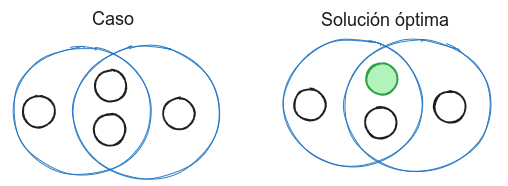
\includegraphics[width=0.8\textwidth]{img/greedy_ej1.png}
    \caption{Ejemplo 1}
    \label{fig:greedy_ej1}
\end{figure}

\begin{figure}[H]
    \centering
    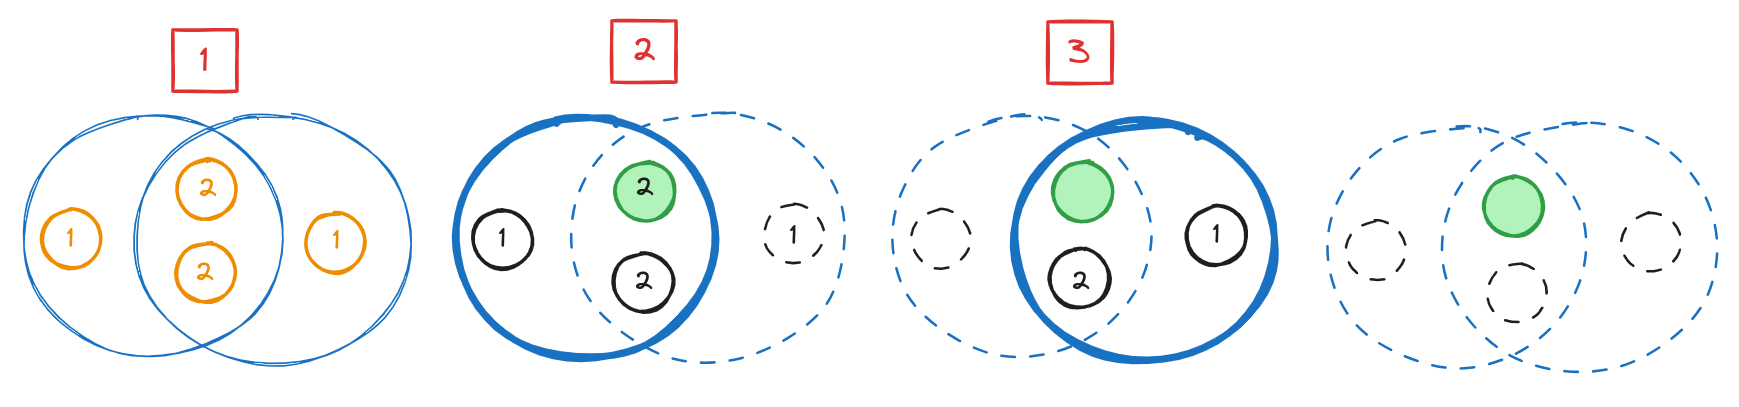
\includegraphics[width=0.8\textwidth]{img/greedy_ej1_mpg.png}
    \caption{Ejemplo 1 resuelto por Máximo por grupo}
    \label{fig:greedy_ej1_mpg}
\end{figure}

\begin{figure}[H]
    \centering
    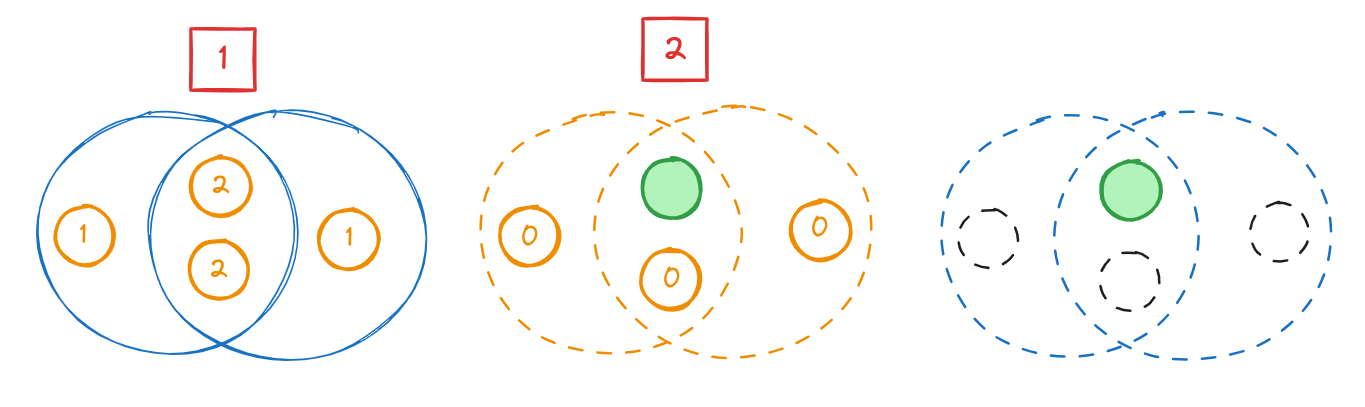
\includegraphics[width=0.8\textwidth]{img/greedy_ej1_mgr.png}
    \caption{Ejemplo 1 resuelto por Máximo global con recálculo}
    \label{fig:greedy_ej1_mgr}
\end{figure}

El segundo ejemplo (fig. \ref{fig:greedy_ej2}) podemos observar en la fig. \ref{fig:greedy_ej2_mpg} que "Máximo por grupo", de menor complejidad, no encuentra la solución óptima, pero el "Máximo global con recálculo", en la fig. \ref{fig:greedy_ej2_mgr}, si.

\begin{figure}[H]
    \centering
    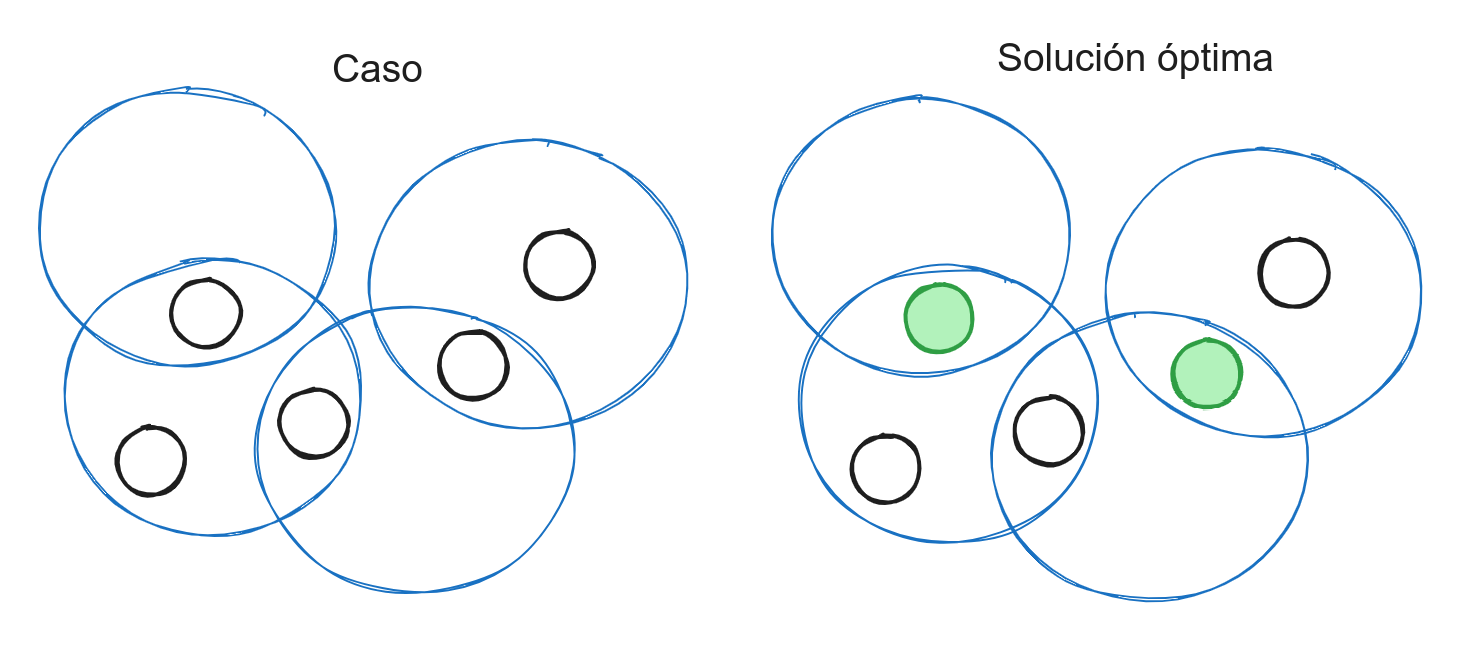
\includegraphics[width=0.8\textwidth]{img/greedy_ej2.png}
    \caption{Ejemplo 2}
    \label{fig:greedy_ej2}
\end{figure}

\begin{figure}[H]
    \centering
    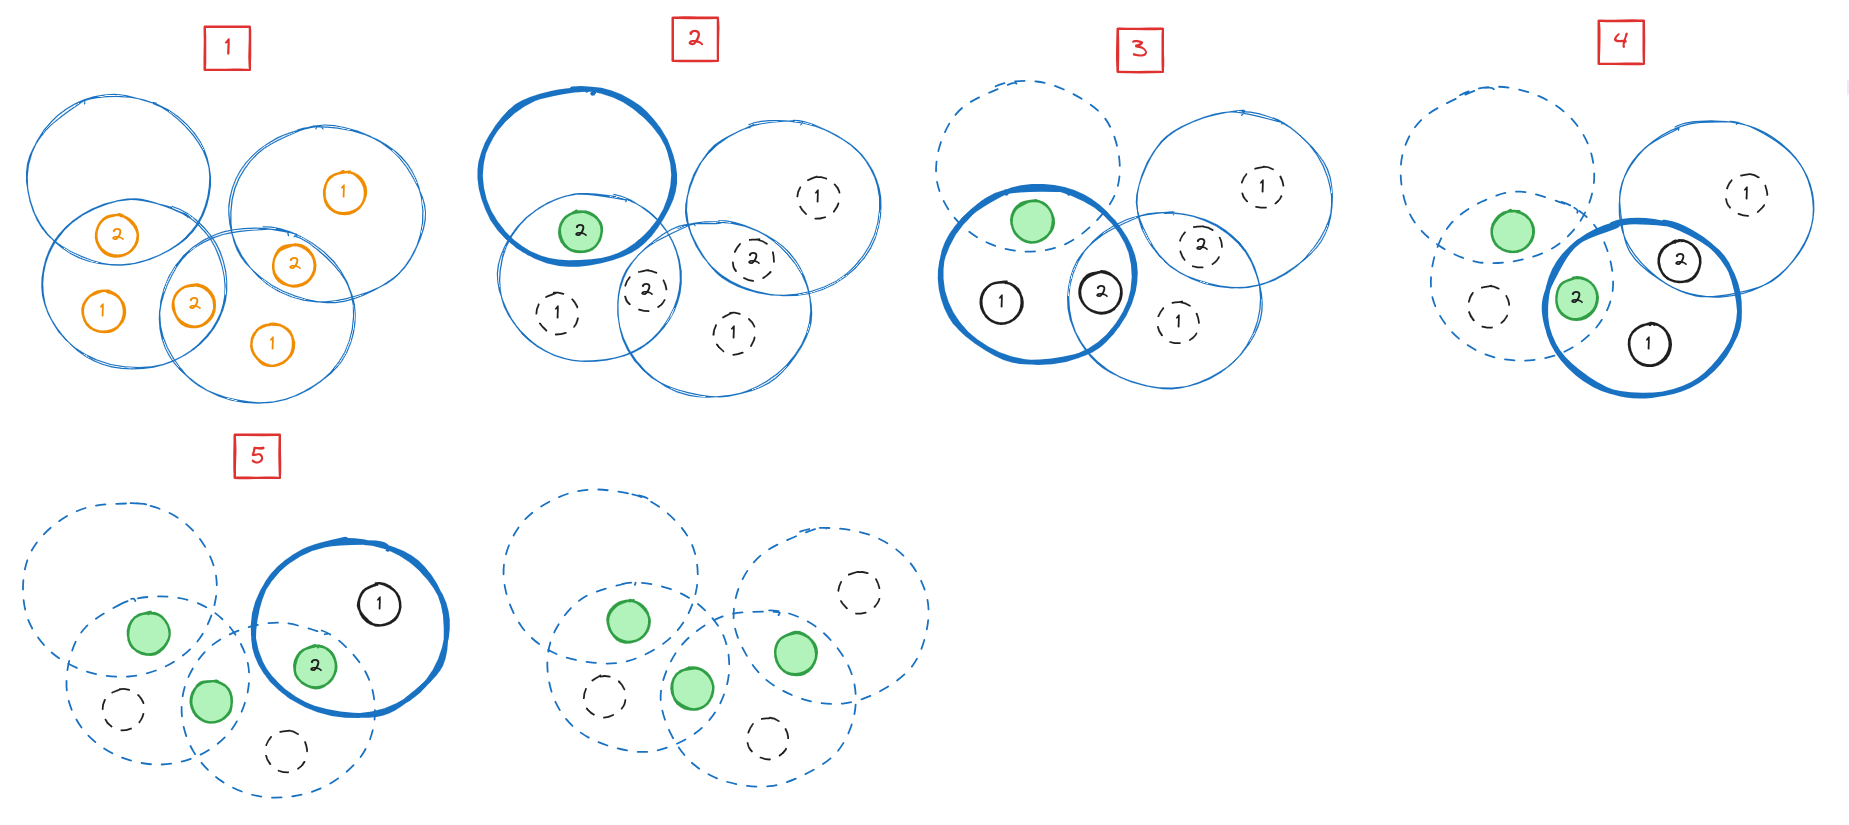
\includegraphics[width=0.8\textwidth]{img/greedy_ej2_mpg.png}
    \caption{Ejemplo 2 resuelto por Máximo por grupo}
    \label{fig:greedy_ej2_mpg}
\end{figure}

\begin{figure}[H]
    \centering
    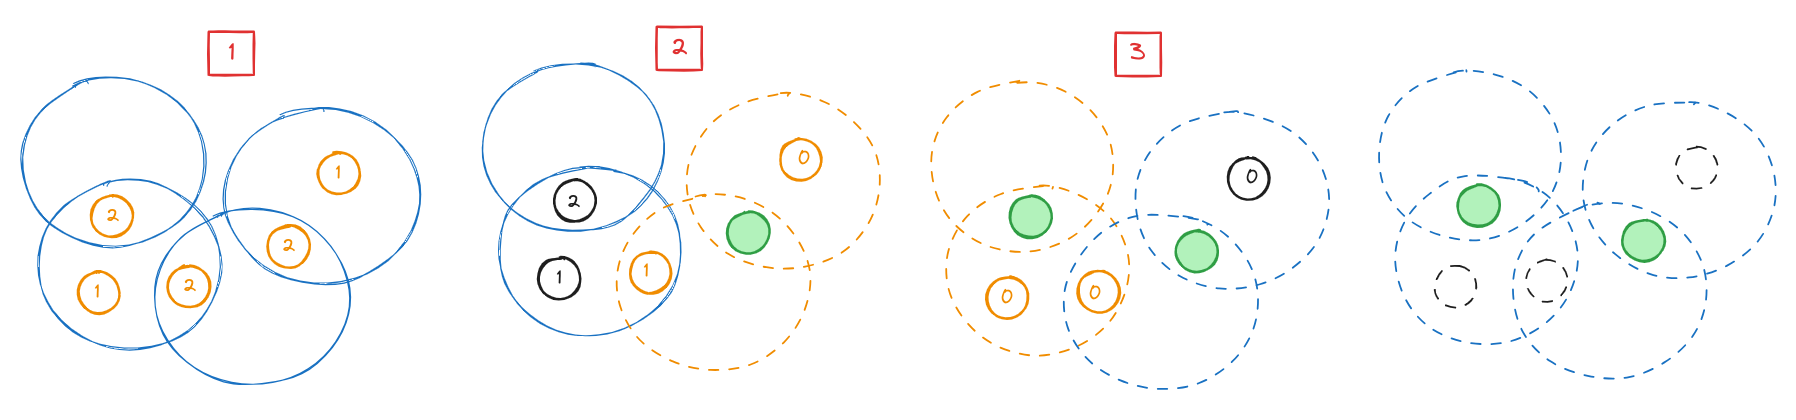
\includegraphics[width=0.8\textwidth]{img/greedy_ej2_mgr.png}
    \caption{Ejemplo 2 resuelto por Máximo global con recálculo}
    \label{fig:greedy_ej2_mgr}
\end{figure}

Por último, en el ejemplo de la fig. \ref{fig:greedy_ej3}, tanto "Máximo por grupo" (fig. \ref{fig:greedy_ej3_mpg}) como "Máximo global con recálculo" (fig. \ref{fig:greedy_ej3_mgr}) no llegan al la solución óptima.

\begin{figure}[H]
    \centering
    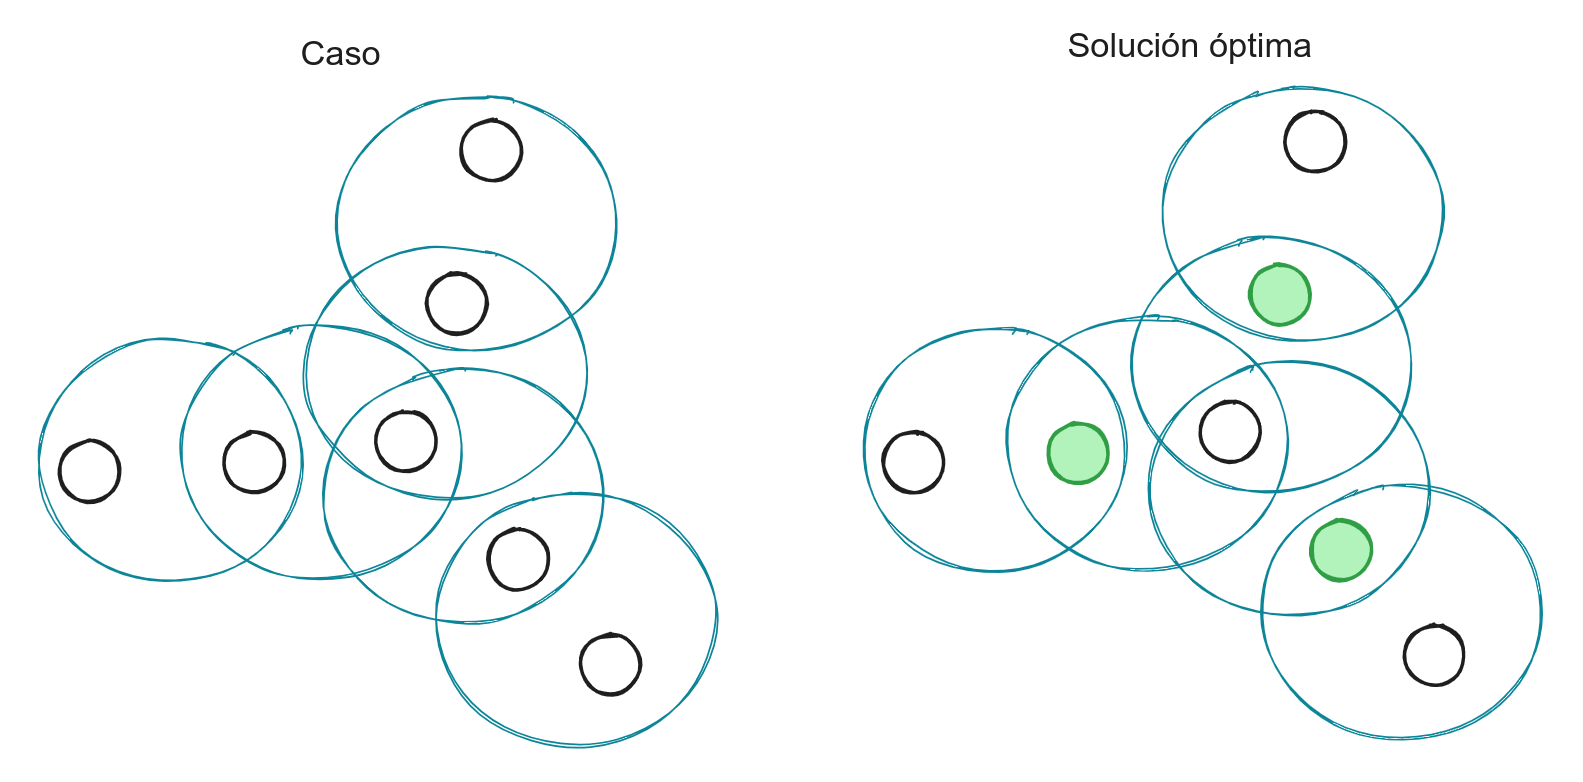
\includegraphics[width=0.8\textwidth]{img/greedy_ej3.png}
    \caption{Ejemplo 3}
    \label{fig:greedy_ej3}
\end{figure}

\begin{figure}[H]
    \centering
    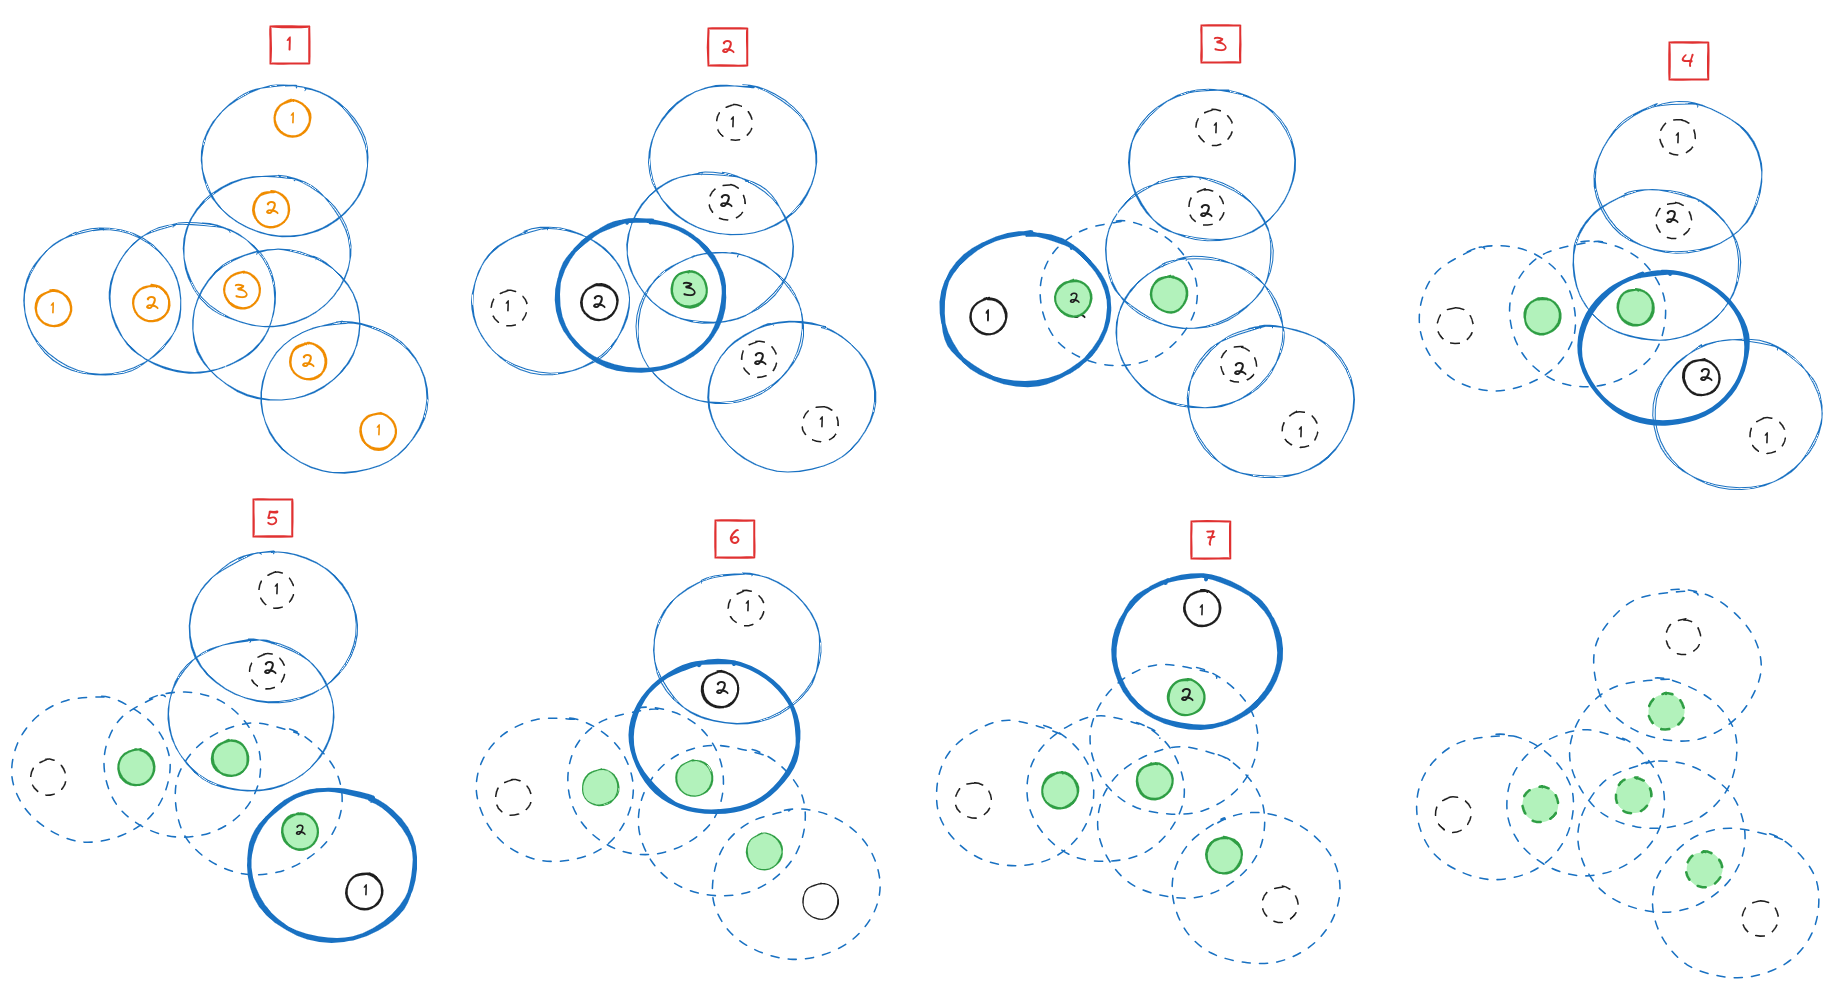
\includegraphics[width=0.8\textwidth]{img/greedy_ej3_mpg.png}
    \caption{Ejemplo 3 resuelto por Máximo por grupo}
    \label{fig:greedy_ej3_mpg}
\end{figure}

\begin{figure}[H]
    \centering
    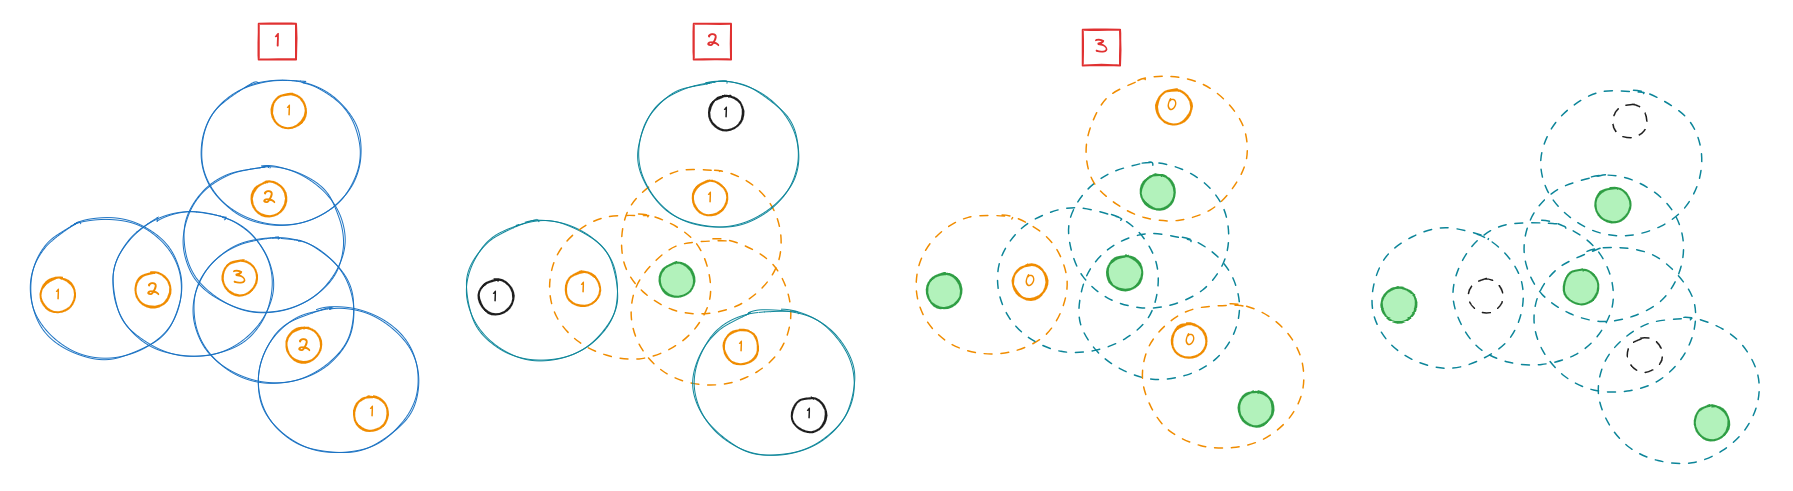
\includegraphics[width=0.8\textwidth]{img/greedy_ej3_mgr.png}
    \caption{Ejemplo 3 resuelto por Máximo global con recálculo}
    \label{fig:greedy_ej3_mgr}
\end{figure}
\section{Conclusiones}

Finalmente, consideramos que la solución óptima para abordar la problemática de Scaloni sería que
éste analizara los compilados en función del tiempo requerido por los asistentes para vi\-sualizar
cada uno, organizándolos en orden descendente.
Esta estrategia permitiría resolver el problema con una complejidad algorítmica de orden 
$\operatorname{O}(n\log{n})$.
Este enfoque garantiza la máxima eficiencia en la visualización de los compilados y permite que el 
tiempo invertido por Scaloni y sus asistentes se administre de manera óptima.


\newpage
\end{document}